\subsection{Arsitektur \textit{Event-Driven}}

\begin{figure}[htbp]
    \centering
    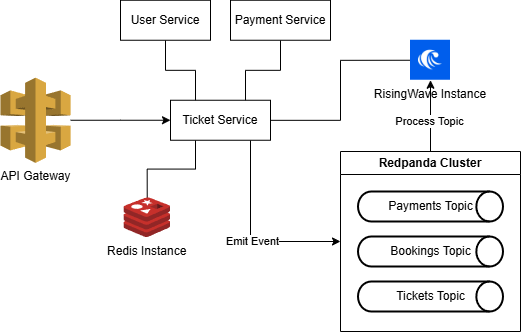
\includegraphics[width=0.8\textwidth]{resources/chapter-3/architecture-event-driven.png}
    \caption{Arsitektur \textit{Event-Driven}}
    \label{fig:solution-event-driven-architecture}
\end{figure}

Arsitektur ini tidak menggunakan PostgreSQL sama sekali. Pada dasarnya, basis data relasional terdiri atas komponen \textit{storage} dan \textit{query processor}. Pada arsitektur ini, komponen \textit{storage} diganti menggunakan Redpanda dengan berbagai topik dan \textit{query processor} diganti dengan RisingWave. Meskipun begitu, pendekatan ini tidak memiliki dukungan \textit{transaction} selain \textit{transaction} pada Redpanda yang berupa \textit{push log all or nothing} pada beberapa topik sekaligus. Untuk itu, Redis digunakan untuk menyimpan \textit{dirty data} atau \textit{uncommited data} sehingga untuk mencegah \textit{double booking}.

Redpanda dapat dibuat kluster dengan pemartisian data untuk meningkatkan \textit{throughput}. Selain itu, RisingWave merupakan \textit{streaming database} yang \textit{cloud-native} sehingga dapat di-\textit{scale out} dengan mudah untuk meningkatkan \textit{throughput}.

Isu \textit{persistence} Redis pada arsitektur ini lebih penting daripada arsitektur sebelumnya. Meskipun begitu, penggunaan kluster dan mode AOF masih dianggap cukup dengan konfigurasi tambahan. Untuk menjamin \textit{stronger durability}, Redis akan dikonfigurasikan untuk selalu melakukan penulisan langsung setelah perintah dijalankan (\texttt{appendfsync always}). Konfigurasi ini akan melakukan penulisan langsung setelah perintah dijalankan. Berbeda dengan konfigurasi \textit{default} Redis yang baru melakukan operasi tulis setiap detik. Kluster Redis masih digunakan untuk \textit{sharding}, tetapi replika tidak akan digunakan untuk menghindari \textit{stale read} karena replikasi pada Redis bersifat asinkron.

